\synctex=1
\documentclass[a4paper,11pt,svgnames]{book}

\usepackage[utf8x]{inputenc}
\usepackage{mathtools}
\usepackage{thesis}
\usepackage{calc}
\usepackage{float}
\usepackage{acronym}
% \setlength{\marginparwidth}{2cm}
% \setlength{\voffset}{-0.25in}
\setlength{\parskip}{0.1in}

\usepackage{todonotes}
\newcommand{\todoin}[1][]{\todo[inline, #1]}

%\includeonly{5-architecture}
%\includeonly{6-use-case}

%\usepackage{draftwatermark}
%\SetWatermarkScale{4}
\usepackage{subfig}
 \usepackage{listings}
  \usepackage{courier}
 \lstset{
 		 basicstyle=\footnotesize\ttfamily,
         numbers=none,               % Ort der Zeilennummern
         numberstyle=\tiny,          % Stil der Zeilennummern
         %stepnumber=2,               % Abstand zwischen den Zeilennummern
         numbersep=5pt,              % Abstand der Nummern zum Text
         tabsize=2,                  % Groesse von Tabs
         extendedchars=true,         %
         breaklines=true,            % Zeilen werden Umgebrochen
         keywordstyle=\color{red},
    	 frame=single,         
 %        keywordstyle=[1]\textbf,    % Stil der Keywords
 %        keywordstyle=[2]\textbf,    %
 %        keywordstyle=[3]\textbf,    %
 %        keywordstyle=[4]\textbf,   \sqrt{\sqrt{}} %
         stringstyle=\color{white}\ttfamily, % Farbe der String
         showspaces=false,           % Leerzeichen anzeigen ?
         showtabs=false,             % Tabs anzeigen ?
         belowcaptionskip=5pt, 
         xleftmargin=2em, 
         xrightmargin=0.8em,
         %backgroundcolor=\color{lightgray},
         showstringspaces=false      % Leerzeichen in Strings anzeigen ?        
 }
 \lstloadlanguages{% Check Dokumentation for further languages ...
         %[Visual]Basic
         %Pascal
         %C
         %C++
         %XML
         %HP
         Java
 }
 
%\usepackage{xcolor}
\usepackage[usenames,dvipsnames,table]{xcolor}

\colorlet{punct}{red!60!black}
\definecolor{background}{HTML}{FFFFFF}
\definecolor{delim}{RGB}{20,105,176}
\colorlet{numb}{magenta!60!black}

\lstdefinelanguage{json}{
    basicstyle=\scriptsize\ttfamily,
    numbers=left,
    numberstyle=\scriptsize,
    stepnumber=1,
    numbersep=4pt,
    showstringspaces=false,
    breaklines=true,
    frame=lrtb,
    backgroundcolor=\color{background},
    literate=
     *{0}{{{\color{numb}0}}}{1}
      {1}{{{\color{numb}1}}}{1}
      {2}{{{\color{numb}2}}}{1}
      {3}{{{\color{numb}3}}}{1}
      {4}{{{\color{numb}4}}}{1}
      {5}{{{\color{numb}5}}}{1}
      {6}{{{\color{numb}6}}}{1}
      {7}{{{\color{numb}7}}}{1}
      {8}{{{\color{numb}8}}}{1}
      {9}{{{\color{numb}9}}}{1}
      {:}{{{\color{punct}{:}}}}{1}
      {,}{{{\color{punct}{,}}}}{1}
      {\{}{{{\color{delim}{\{}}}}{1}
      {\}}{{{\color{delim}{\}}}}}{1}
      {[}{{{\color{delim}{[}}}}{1}
      {]}{{{\color{delim}{]}}}}{1},
}
    %\DeclareCaptionFont{blue}{\color{blue}} 

  %\captionsetup[lstlisting]{singlelinecheck=false, labelfont={blue}, textfont={blue}}
  \usepackage{caption}
%\DeclareCaptionFont{white}{\color{white}}
%\DeclareCaptionFormat{listing}{\colorbox[HTML]{6DBAFF}{\parbox{\textwidth}{\hspace{5pt}#1#2#3}}}

\DeclareCaptionFont{white}{\color{white}}
\DeclareCaptionFormat{listing}{\colorbox{gray}{\parbox{\textwidth-20pt}{#1#2#3}}\vspace{0.01cm}}
\captionsetup[lstlisting]{format=listing,labelfont=white,textfont=white}

\captionsetup[lstlisting]{format=listing,labelfont=white,textfont=white, singlelinecheck=false, margin=0pt, font={bf,footnotesize}}


\usepackage{url}

%\usepackage[spanish]{babel}
%\usepackage[T1]{fontenc}
\usepackage{tabularx}
\usepackage{graphicx}
%\usepackage[usenames,dvipsnames,table]{xcolor}
\usepackage{verbatim}
\usepackage[section]{placeins}
\usepackage{listings}
%\bibliographystyle{unsrt}


\newcommand{\authorname}{Ignacio Cervantes Villalón}
\newcommand{\tfgtitle}{Desing and development of chatbot trained with machine learning models}
\newcommand{\tfgtitlees}{Diseño e implementación de un chatbot entrenado mediante modelos de machine learning}
\newcommand{\tutor}{Carlos Ángel Iglesias Fernández}
\newcommand{\supervisor}{PONENTE}
\newcommand{\fecha}{MES 20XX}

\usepackage[pdftex,
    pdfauthor={\authorname},
            pdftitle={\tfgtitle},
            pdfsubject={Master Final Project},
            pdfkeywords={GSI},
            pdfproducer={PDFTex},
            colorlinks=true,linkcolor=black,citecolor=black,urlcolor=black,hypertexnames=false]{hyperref}

%\usepackage{longtable}
\setcounter{secnumdepth}{3}

\usepackage{framed}

%lstlisting
\usepackage{listings}

\lstdefinelanguage{JavaScript}{
  keywords={typeof, new, true, false, catch, function, return, null, catch, switch, var, if, in, while, do, else, case, break},
  keywordstyle=\color{blue}\bfseries,
  ndkeywords={class, export, boolean, throw, implements, import, this},
  ndkeywordstyle=\color{darkgray}\bfseries,
  identifierstyle=\color{black},
  sensitive=false,
  comment=[l]{//},
  morecomment=[s]{/*}{*/},
  commentstyle=\color{purple}\ttfamily,
  stringstyle=\color{red}\ttfamily,
  morestring=[b]',
  morestring=[b]"
}

\definecolor{darkblue}{rgb}{0.0,0.0,0.6}

\lstdefinestyle{listXML}{language=XML, basicstyle=\ttfamily\diny, extendedchars=true,  belowcaptionskip=5pt,xleftmargin=0.4em, xrightmargin=0.3em, numbers=none, frame=single, breaklines=true, breakatwhitespace=true, breakindent=0pt, emph={}, emphstyle=\color{red}, basicstyle=\small\ttfamily, columns=fullflexible, showstringspaces=false, commentstyle=\color{gray}\upshape,
morestring=[b]",
morecomment=[s]{<?}{?>},
morecomment=[s][\color{orange}]{<!--}{-->},
keywordstyle=\color{cyan},
stringstyle=\color{black},
tagstyle=\color{darkblue},
morekeywords={xmlns,version,type}
}



\lstdefinestyle{mono}{
   framesep=8px,
   extendedchars=true,
   basicstyle=\ttfamily,
   showstringspaces=false,
   showspaces=false,
   tabsize=2,
   breaklines=true,
   showtabs=false,
   xleftmargin=8pt,
   xrightmargin=8pt
}


\lstdefinestyle{commands}{
   framesep=8px,
   extendedchars=true,
   basicstyle=\ttfamily,
   showstringspaces=false,
   showspaces=false,
   tabsize=2,
   breaklines=true,
   showtabs=false,
   xleftmargin=8pt,
   xrightmargin=8pt
}

\lstdefinestyle{consola}
   {basicstyle=\scriptsize\ttfamily,
    backgroundcolor=\color{white},
    frame=lrtb,
    numbers=none,
    xleftmargin=4pt,
    xrightmargin=4pt
   }

% Allows to change the color of chapter headers
\definecolor{chapterdetails}{HTML}{00a9e0}

% \usepackage[sf,bf]{titlesec}
% \titleformat{\chapter}[display]
%   {\normalfont\Large\sffamily\raggedleft}
%   {\vspace{5cm}\MakeUppercase{\chaptertitlename}%
%     \rlap{ \resizebox{!}{1.5cm}{\thechapter} \color{chapterdetails}\rule{5cm}{1.5cm}}}
%   {10pt}{\Huge}[{\color{chapterdetails}\titlerule[0.8mm] }]
% \titlespacing*{\chapter}{0pt}{30pt}{20pt}

\usepackage[sf,bf]{titlesec}
\titleformat{\chapter}[display]
  {\normalfont\Large\sffamily\raggedleft}
  {\vspace{5cm}\MakeUppercase{\chaptertitlename}%
    \rlap{ \resizebox{!}{1.5cm}{\thechapter} \color{chapterdetails}\rule{5cm}{1.5cm}}}
  {10pt}{\Huge}[{\color{chapterdetails}\titlerule[0.8mm] }]
\titlespacing*{\chapter}{0pt}{30pt}{20pt}

%\titleformat{\section}{\large\sffamily\bfseries}{\thesection}{1em}{}


\newenvironment{chapterintro}
{% This is the begin code
\large\it
}
{% This is the end code
}


% Tick symbols
\newcommand{\tickYes}{\checkmark}
\newcommand{\tickNo}{\hspace{1pt}\ding{55}}
% Fancy header
\usepackage{fancyhdr}
%Fancy chapter cover style


% Fancy box
\usepackage{fancybox} 
\setlength{\fboxrule}{1 pt} \setlength{\fboxsep}{10pt} \setlength{\shadowsize}{3pt}

%Sky color definition

%% Portada
\usepackage{eso-pic,graphicx}
\usepackage{chngpage}
% \usepackage{tikz}
% \usepackage[top=0cm, bottom=0cm, outer=0cm, inner=0cm]{geometry}


\begin{document}
\newcommand\litem[1]{\item{\bfseries #1 }}
\renewcommand{\arraystretch}{1.5} %Makes tables less crammed

\newcommand\headcell[1]{%
  \multicolumn{1}{|c|}{\cellcolor{DodgerBlue}\bfseries\sffamily\textcolor{white}{#1}}
}

%%%%% ACRONYM DEFINITION
\acrodef{nlp}[NLP]{\emph{Natural Language Processing}}
\acrodef{ai}[AI]{\emph{Artificial Intelligence}}
\acrodef{ar}[AR]{\emph{Augmented Reality}}
\acrodef{tas}[TAS]{\emph{Task Automation Service}}
\acrodef{vpa}[VPA]{\emph{Virtual Private Assistant}}
\acrodef{pos}[POS]{\emph{Parts Of Speech}}
%Cuadros por tablas
%\renewcommand{\listtablename}{Tables Index}
%\renewcommand{\tablename}{Table} 

% \renewcommand{•}{•}*{\lstlistingname}{List of X}
	
\pagenumbering{Roman}

\pagestyle{empty}
% \tikz[remember picture,overlay] \node[opacity=1,inner sep=0pt] at (current page.center){
\includegraphics[height=\paperheight]{img/portada.png}};

\vspace*{5.5cm}

\begin{center}

{\Large\rm \textbf{ MÁSTER UNIVERSITARIO EN\\
INGENIERÍA DE TELECOMUNICACIÓN\\}}

\vspace{1.0cm}

{\Large\rm \textbf{TRABAJO FIN DE MASTER}}

\vspace{2cm}

{\Large\rm\textbf{\tfgtitle}}

\vspace*{\fill}

{\Large\rm\textbf{IGNACIO CERVANTES VILLALÓN}}

{\Large \textbf{2020}}
\vspace{1.0cm}
\end{center}
\AddToShipoutPictureBG*{
\includegraphics[width=\paperwidth,height=\paperheight]{docs/img/portada.png}}

\cleardoublepage
\thispagestyle{empty}
\vspace*{3\baselineskip}
{\large{\bf TRABAJO DE FIN DE MASTER}}
\vspace{0.5cm}

\begin{rm}
\begin{tabular}{p{3cm}p{10cm}}
\textbf{Título:} & \tfgtitlees \\ 

\textbf{Título (inglés):} & \tfgtitle \\ 
\textbf{Autor:} & \authorname{} \\ 
\textbf{Tutor:} & \tutor \\ 
\textbf{Ponente:} & \supervisor \\ 
\textbf{Departamento:} & Departamento de Ingeniería de Sistemas Telemáticos \\ 
\end{tabular} \end{rm} \vspace{1cm}

{\large{\bf MIEMBROS DEL TRIBUNAL CALIFICADOR}} \vspace{0.5cm}

\begin{rm}
\begin{tabular}{p{3cm}p{10cm}}
\textbf{Presidente:} & -----\\
\textbf{Vocal:} & -----\\
\textbf{Secretario:} & -----\\
\textbf{Suplente:} & -----
\end{tabular}
\end{rm}
\vspace{1cm}

{\large{\bf FECHA DE LECTURA:}}
\vspace{1cm}

{\large{\bf CALIFICACIÓN:}}
\pagestyle{empty}
\cleardoublepage
\vspace*{\baselineskip}
\begin{center}
	{\LARGE\rm\textbf{UNIVERSIDAD POLITÉCNICA DE MADRID}\\
	\vspace{1.0cm}
	 ESCUELA TÉCNICA SUPERIOR DE\\ INGENIEROS DE TELECOMUNICACIÓN
	  }  \\

	 {\Large\rm Departamento de Ingeniería de Sistemas Telemáticos\\
	 Grupo de Sistemas Inteligentes  }  \\

\begin{figure}[!htbp]
	\centering
    
\includegraphics[width=0.7\textwidth]{img/logo_etsit.jpg}

\end{figure}
	\vspace{1.0cm}
	{\LARGE\rm TRABAJO DE FIN DE MASTER\\
	\vspace{2.0cm}
    \tfgtitle
	 \vspace{0.5cm}}
	 
	 \vspace{1.0cm}
     \Large\rm\textbf{\author}\\
	 \vspace{1.0cm}
     \fecha
\end{center}  

%\cleardoublepage
%
%\begin{tabular}{p{10cm}p{4cm}}
%&\\
%&\\
%&\\
%&\\
%&\\
%&\\
%&\\
%&\\
%&\\
%&\emph{Write cool quote here}\\
%&\\
%\end{tabular}
\cleardoublepage
\phantomsection
\chapter*{Resumen}
\addcontentsline{toc}{chapter}{Resumen}
En los tiempos que corren, la interacción con sistemas automáticos es una parte fundamental a la hora de realizar tareas cotidianas en sistemas informáticos. Realizar una gestión sobre un pedido en una tienda online o solicitar asistencia técnica son algunas de las aplicaciones suelen recaer en automatismos para ofrecer una respuesta rápida, acotada y certera. En este contexto, los llamados Chatbots, consistentes en una inteligencia artificial capaz de simular el comportamiento conversacional de una persona, permiten ofrecer una interfaz amigable para automatizar tareas. El objetivo de este TFM es el de desarrollar un caso de estudio de la aplicación de un chatbot para llevar a cabo el servicio de atención al consumidor. El objetivo de este TFM es estudiar el panorama de los chatbot en la actualidad, mostrando su evolución desde sus inicios hasta el día de hoy comparando sus características y mostrar un caso práctico implantando uno de ellos. Para profundizar en el estudio, se va a desarrollar un caso práctico de uso del chatbot de código libre RASA, haciendo uso de técnicas de machine learning para entrenar sus modelos y comparando los resultados obtenidos mediante la conversación con el robot. Se pretende con ello ver las posibilidades de evolución de un chatbot al involucrar aprendizaje en el modelo de conversación del robot, y comparar los resultados obtenidos con los distintos algoritmos utilizados. Para ello se utilizará Jupyter Notebook y Python.
\vfill
\textbf{Palabras clave:} Chatbot, RASA, Machine Learning, Python.
\cleardoublepage
\phantomsection
\chapter*{Abstract}
\addcontentsline{toc}{chapter}{Abstract}
Nowadays, interaction with automatic systems is a fundamental part in order to perform day-to-day tasks in informatic systems. Managing an online shop order or asking for technical assistance are some of the applications where automatisms can offer a fast and precise response. In this context, the so-called Chatbots, that consist in an AI capable of simulating an human-like conversation, can offer a friendly user interface to automatize these tasks. This TFM objective is to develop a case of study of a chatbot applicated to a customer service. In order to do this, a practical case of a open-source code chatbot called RASA is proposed, using machine learning techniques to train its models, comparing the results obtained in a conversation with the bot. The objective is to check the possibilities of evolution that chatbot when machine learning in the conversational model is involved, and compare the results of different machine learning algorithms. The development will be done using RASA as the chatbot where we are going to develop the use case, Jupyter Notebook to make human-friendly code and keep the results organized, Python 3.8 to run the algorithms, notebooks and RASA. 
\vfill
\textbf{Keywords: }Chatbot, RASA, Machine Learning, Python 
%\cleardoublepage
\phantomsection
\addcontentsline{toc}{chapter}{Acknowledgement}

\begin{center}
\textbf{\large Acknowledgement}
\end{center}

Acknowledgement
\cleardoublepage
\phantomsection
\chapter*{Agradecimientos}
\addcontentsline{toc}{chapter}{Agradecimientos}

A Gauss

\cleardoublepage
\phantomsection
\addcontentsline{toc}{chapter}{Contents} % para que aparezca en el indice de 
\tableofcontents % indice de contenidos


\cleardoublepage
\phantomsection
\addcontentsline{toc}{chapter}{List of Figures} % para que aparezca en el indice de contenidos
\listoffigures % indice de figuras

%\cleardoublepage
%\phantomsection
%\addcontentsline{toc}{chapter}{List of Tables} % para que aparezca en el indice de contenidos
%\listoftables % indice de tablas

\cleardoublepage


%Header style
\pagestyle{fancy}
\fancyhf{}
\fancyhead[RO]{\sffamily \slshape \rightmark}
\fancyhead[LE]{\sffamily \slshape \leftmark}
%\renewcommand{\footrulewidth}{0.4pt} % grosor de la línea del pie
\fancyfoot[OR,EL]{\rmfamily \thepage} % texto derecha del pie
\pagenumbering{arabic}

\chapter{Introduction}

\section{Context}

Nowadays, it is common to interact with business to request services such as technical attention or responses with advise using their products. Interacting in social networks such as Twitter or Facebook is a familiar way to users to get in touch with the support they need. For example, telecommunication service providers such as Movistar or Orange can be reached quickly by writing a message in a social media, instead of a complicated and usually longer telephonic conversation. In these situations, getting a fast response can mean the difference between a happy customer or losing it.

In this scenario, is desirable automatizing as much as possible to offer a quick response and save costs. To do this and offer a person-like behavior, a common solution is deploying a chatbot. This way, the service provider can give the user a way of getting the information needed in a friendly environment.


\clearpage

\section{Project goals}

Describe the different goals of the project


\clearpage

\section{Structure of this document}

The remaining of this document is structured as follows:

\textbf{\textit{Chapter 2}} ... (Chapter 1 is the Introduction)
\chapter{State of Art}
\label{chap:state-of-art}
\textit{Introduction of the state of art}

\clearpage

\section{Sentiment Analysis}

\clearpage

\section{Neural Networks}


\chapter{Enabling Technologies}
\label{chap:enabling_technologies}

\textit{This  chapter  offers  a  brief  review  of  the  main  technologies  that  have  made  possible this  project. For the realisation of this TFM, Python is the main programming language. To make it easier to track, Jupyter Notebook is used. Jupyter allows the user to execute the code in cells and see the results for each one, that makes simpler reading the code.
To develop the chatbot, the open-source framework RASA is used. RASA allows to develop a chatbot, train its models with machine learning and improve the performance through analysing conversation with RASA X. The following sections explain the fundamentals of these packages and others that are used in the consecution of this project.}
\clearpage

\section{Introduction}
To develop this project, many technologies are involved that need to be understood to. In this chapter, we are going to analyze and explain some of them to offer a wider vision of how the project is achieved. 

First of all, we are going to explain the technology behind the applications that are used in this project, Cognitive computing. We will deepen in the definition and explain some of its characteristics, as well as list some of their applications.

Secondly, we will analyse the conversational bots by its characteristics, and offer a wide vision of the different applications that are being used now. The chatbots that we are going to cover are IBM Watson, Google Dialogflow and RASA.

Finally, we are going to give conclusions about this chapter.

\section{Cognitive computing}

As artificial intelligence and new ways of programming grow, the principal companies have found new advantages in their usage. IBM, Microsoft or Facebook are making great investment in this technologies to make their companies more relevant, and take a leap to cognitive applications. "Cognitive computing" is a term that has been in the sector for years with different definitions. As stated by the Cognitive Computing Consortium\cite{cognitive_definition}, a cross disciplinary group of experts, cognitive computing may be defined as:

\textsl{"Cognitive computing makes a new class of problems computable. It addresses complex situations that are characterized by ambiguity and uncertainty; in other words it handles human kinds of problems. In these dynamic, information-rich, and shifting situations, data tends to change frequently, and it is often conflicting. The goals of users evolve as they learn more and redefine their objectives. To respond to the fluid nature of users’ understanding of their problems, the cognitive computing system offers a synthesis not just of information sources but of influences, contexts, and insights. To do this, systems often need to weigh conflicting evidence and suggest an answer that is “best” rather than “right"".}

Unlike current computing paradigms, cognitive computing model infers some data that is out of scope for basic computing. This way, cognitive computing makes context computable, taking account and using some state-of-the-art technologies like machine learning, natural language processing or feature engineering. In other words, as the Cognitive Computing Consortium states, cognitive computing applications "suggest an answer that is "best" rather than "right"".

To sum up, cognitive computing aims to endow computer systems with the faculties of knowing, thinking and feeling\cite{cognitive_gutierrez_garcia} to close the gap between people and the informatic environment. For this reason, it is the basis of technologies like virtual assistants or chatbots. However, it is thought that new applications of cognitive computing will appear in other fields of knowledge.

\subsection{Cognitive computing properties}


As the Cognitive Computing Consortium states, there are some features that a cognitive system has to fulfil: 
\begin{itemize}
    \item \textbf{Adaptive:} They must be capable of learning as information and goals evolve. They must resolve ambiguity and tolerate unpredictability. Also, they must be engineered to feed on dynamic data in real time, or near real time.
    \item \textbf{Interactive:} A cognitive system must be easy to interact with, so the users can define their needs and requirements in a simple way. They may also be capable of interact with other actors and devices as other users, Cloud services or online applications.
    \item \textbf{Iterative and stateful:} They must be capable to aid the user in defining a problem by asking questions or finding additional source input if a problem statement is ambiguous or incomplete. They must take in consideration previous interactions in a process and return information that is suitable for the specific application at that point in time
    \item \textbf{Contextual:} They must be capable of understand and extract contextual elements of the information, such as meaning, syntax or time. Also, they may be able to obtain information from various sources, structured or not, as well as sensory inputs if the system support them.
\end{itemize}

\subsection{Use Case of Cognitive Systems}
As cognitive systems advance, more and more applications that uses them appear and their relevance rises. Some of the most relevant use cases are:
\begin{itemize}
    \item \textbf{\acf{vpa}:} \acp{vpa}\cite{rise_of_bots} are \acl{ai} applications that assist the user utilizing their devices. They act as an "human-like" interface to perform some tasks, launched by the user by giving orders to the assistant via voice or text.
    
    Most \acp{vpa} are present in several devices and offer services such as access to device functions as making a phone call or writing a message, appointment management or domotic control, and they are linked to personal accounts to take in consideration user's profile and preferences. Some of the most popular are Apple's Siri, Google Assistant, Microsoft's Cortana or Amazon Alexa.
    \item \textbf{Augmented reality:} \acf{ar} technology is a variation of virtual environments where the user is able to see the real world with virtual objects composited in it. Therefore, \acs{ar} "supplements reality, rather than replacing it"\cite{augmented_reality_survey}. 
    
    \acs{ar} applications take information from cameras to put into the captured images 3D models or layers of information that are reactive to the environment and are capable of adapt to it. These applications can run on various devices, being the most typical smartphones or \textsl{Head Mounted Devices (HMD)} such as Microsoft Hololens\cite{microsoft_hololens}.
    \begin{figure}[ht]
    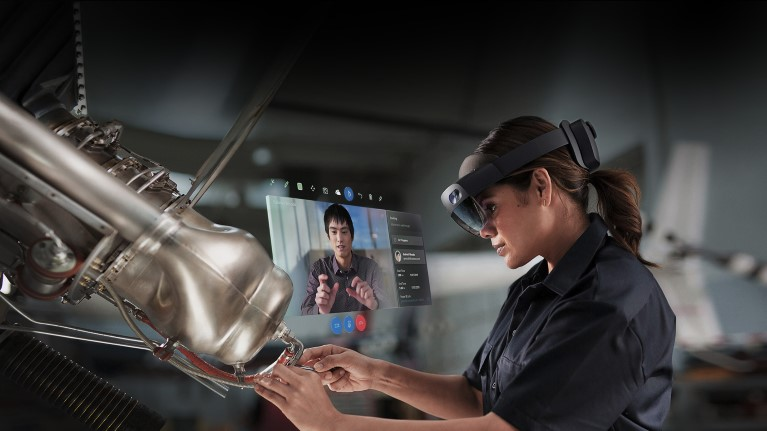
\includegraphics[scale=0.6]{docs/img/project_pics/hololens.jpg}
    \centering
    \caption{Person using Microsoft Hololens \cite{hololens_pic}}
    \end{figure}

    
    Some of the applications of this technology are engineering, 3D design or videogames such as Pokémon GO.
    \item \textbf{Face recognition:} Face recognition allows to use images capted by a camera to identify a person face. This systems recognize patrons in faces through \acs{ai} to identify univocally a person. 
    
    This technology is widely used in biometric security authentication systems, such as Apple's Face ID, or in social networks like Facebook to tag users automatically by identifying their faces in photographs uploaded by their contacts.
\end{itemize}

\section{Chatbots}
Since the beginning of domestic computers, there was always an interest in giving the user a friendly interface to use the computational resources. Investing in a clear user interface or designing an attractive and simple website makes the user want to use these resources. As the number of people that uses computers rose, it turned to be a necessity that may decide if an application success or fails. In these context, giving the user a natural language interface to interact with is desirable.

As speech is one of the main forms of communication between humans, the researchers aimed to inspire from it. Speech interaction is gaining interest in the past few years, as can be seen from developments from Google, Apple or IBM. 

\textsl{Chatterbots} (or, from now, \textsl{chatbots}) are applications designed to imitate human-like conversation. From the simplest models to modern \acs{ai}-powered, the goal is to offer a more friendly way to the user to interact with a digital system. 

The first recognized chatbot was \textsl{ELIZA}, a program created by Joseph Weizenbam at MIT in 1966, that communicated with humans based on hand-crafted scripts. The conversation scope was limited as it was designed using pattern recognition, but enough to keep a realistic conversation, as can be seen in the figure below.
\begin{figure}[ht]
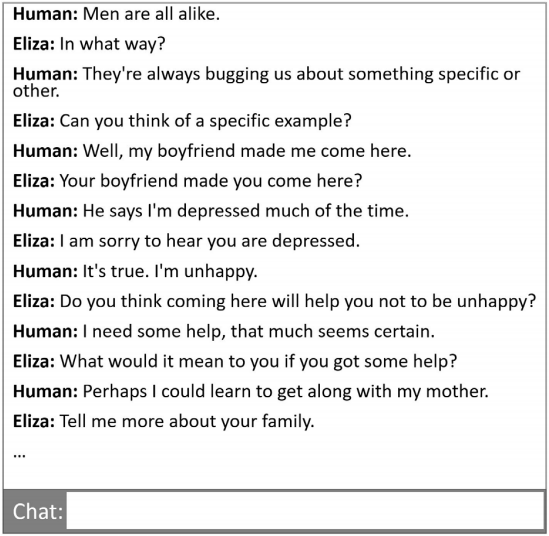
\includegraphics[scale=0.5]{docs/img/project_pics/Eliza.png}
\centering
\caption{Conversation between a person and ELIZA \cite{eliza}}
\end{figure}

Another milestone in chatbot history was Parry, a chatbot developed by Colby designed to have a paranoid behavior in conversation. Parry was the first chatbot that passed the Turing test, that means that it showed a indistinguishable behaviour from a human\cite{turing}. It was also ruled-based as ELIZA, but Parry had a better language understanding capabilities and models that allowed it to mimic human emotions. For example, it was capable of showing hostility if the anger level in conversation was high.

However, the more recent and modern approaches of chatbots are not longer based on pattern recognition. The chatbots that are listed in the next sections are based in \acf{nlp} and machine-learning techniques. 
\subsection{Chatbots Design Techniques}
To be able to give suitable responses to the user inquiries, some programming skills and techniques must be used to program a chatbot. In this section we are going to briefly explain them, as well as understanding the different parts of a chatbot.

As chatbots evolve into more realistic conversational partners, the complexity in programming them also multiplies. For this reason, designing a chatbot require identifying its main parts. A Chatbot can be classified into three main parts\cite{design_techniques}:
\begin{itemize}
    \item \textbf{Responder:} This part acts as the interface between the bot logic and the user. Its goal is to pass the data from the user to the next step and controlling the inputs and outputs of the system.
    \item \textbf{Classifier:} This layer connects the responder and the graphmaster, and is able to filter and normalise the inputs from the user to pass it to the graphmaster. It also processes the output of the graphmaster if needed.
    \item \textbf{Graphmaster:} This part is in charge of the logic of the chatbot. It keeps the storage and performs the operations needed to determinate the response (i.e. pattern matching)
\end{itemize}
\begin{figure}[ht]
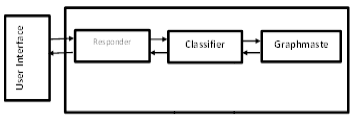
\includegraphics[scale=1]{docs/img/project_pics/chatbot_parts.png}
\centering
\caption{Components of a chatbot \cite{design_techniques}}
\end{figure}

To design a chatbot, some programming techniques and skills are needed. Some of the most important are:
\begin{itemize}
    \item \textbf{Parsing:} Analysing the input text received from the user and manipulate it (i.e. morphemes recognition) with \acs{nlp} functions. 
    \item \textbf{Pattern matching:} Detecting patterns in the user messages to catch the meaning or the sentiment of them, and respond in consonance. 
    \item \textbf{Markov Chain:} It is a stochastic model widely used in chatbots to give responses taking account of previous responses, which means that the next state probability is conditioned by the previous states.
\end{itemize}
\subsection{Chatbot Frameworks}
The number of chatbot frameworks has been increasing since a few years ago, at the same time as they evolved into more interactive and functional tools. The evolution of webs also allowed to embed chatbots into websites to give the visitor a way to interact with the company without having a person 24/7. As many companies noticed how the inclusion of a chatbot made an impact in their economy, the interest for different options rose.

There are many benefits of implementing a chatbot for a company in its website. Having a chatbot usually offers an instantaneous responsive option for an user, reducing support cost. Also, it makes a company easier to operate worldwide, as a chatbot is always operative instead of having to adapt to local hour. In terms of savings, about of 30\% of costs in support can be reduced\cite{saving_percent}.

Chatbots can be found in many different applications and forms. In this section we are going to introduce some of the most important frameworks and chatbots used in the present.

\subsubsection{IBM Watson Conversation}
IBM Watson is a conversation tool, initially designed as a question answering system based on natural language processing, information retrieval, knowledge representation, automated reasoning, and machine learning\cite{ibm_watson}. It can be deployed in cloud services such as IBM Cloud, Amazon Web Services, Azure or Google Cloud, and the service can be developed using different languages SDKs, such as Java or Python. 

As a chatbot, some of the features that Watson offers is to interact with the bot through voice and text. Once the message is sent to the assistant, the content is analysed through the system. As a differential point with other assistants, Watson decides when to search for an answer from a knowledge base, when to ask for clarity and when to escalate the request to a human to resolve it. Also, as it can be deployed in the cloud service that the user decides, the sensible data and conversations are only stored in it, and not collected by the chatbot provider. This allows to train the bot with that data, and preserve the privacy of the users.


\begin{figure}[ht]
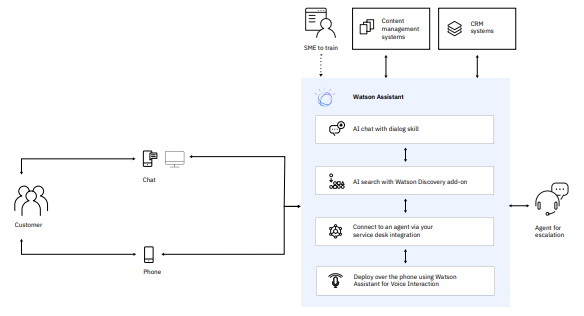
\includegraphics[scale=0.8]{docs/img/project_pics/watson_customer.png}
\centering
\caption{Watson Assistant solution for customer service \cite{watson_diagram}}
\end{figure}


\subsubsection{Dialogflow}
Dialogflow is a conversational tool developed by Google and deployed by Google Cloud. It is based on \acl{nlp} and machine learning techniques, and it is one of the most important conversational AI in the market. Some of their clients are big companies such as Ticketmaster or Domino's Pizza, which uses the chatbot to make orders\cite{dominos}.

Google describes Dialogflow as "an end-to-end, build-once deploy-everywhere suite for creating conversational interfaces"\cite{dialogflow_overview}. Some of its strengths are 

Dialogflow functionality is achieved by different parts that conform the full stack:
\begin{itemize}
    \item \textbf{Agent:} An agent is a virtual entity that handles conversation with the end-user. It interacts in natural language, via text or audio, and is trained to handle expected conversations with the user.
    \item \textbf{Intents:} Every user intention is categorized in "intents". The agent is trained to recognise the differences between them, extract information from them and perform an action as a response. An intent contains \textsl{training phrases}, that are example phrases that the user might send, \textsl{actions} that triggers certain logic in the system, \textsl{parameters} extracted from the user message that can be used through conversation and \textsl{responses}, which continues the conversation with the user. 
    \item \textbf{Intents:} Dictates how data obtained from the user is extracted and managed
    \item \textbf{Contexts:} Interpretation by Dialogflow for the context of the conversation. This allows to match an intent to some specific context to make Dialogflow more likely to match the next intents related to that context, just as human communication works.
    \item \textbf{Fulfillment:} As Dialogflow can integrate other service in order to give a response, fulfillments functions connecting an intent with a call to a service defined. For example, it can match a question about the weather with a search in a database with a weather history.
\end{itemize}
\begin{figure}[ht]
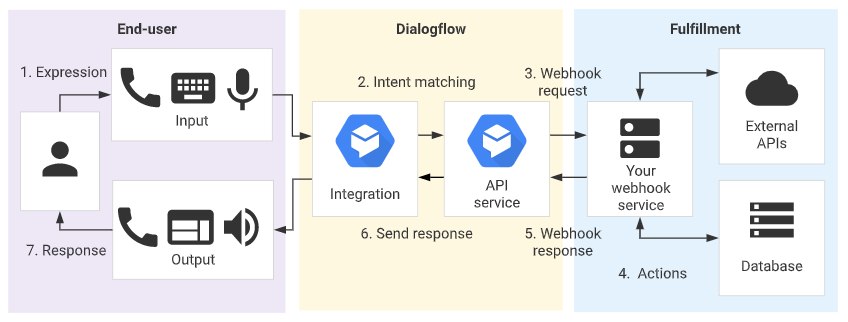
\includegraphics[scale=0.5]{docs/img/project_pics/dialogflow.png}
\centering
\caption{Dialogflow architecture overview \cite{dialogflow_overview}}
\end{figure}

\subsubsection{RASA}
RASA is a conversational AI framework for building contextual assistants. Unlike IBM Watson or Google Dialogflow, RASA is an Open Source alternative, which allows to deploy it on a diverse set of platforms and tune it to the user needs. RASA offers a paid "Enterprise plan" with analytics and support from the company, but the user can get full functionality with the free version.

RASA conversational functionality is based in the context of the conversation. Unlike first pattern-recognition chatbots, where the engine searched for specific word sequences to give a response but did not take in consideration the surrounding information of the conversation, contextual assistants can handle a conversation in a more human-like way, making the correct questions to get the information needed to fulfill more complex needs. 

RASA's architecture is modular, allowing to easily integrate with other systems. As it is coded in Python and makes use of standard libraries such as \textsl{scikit-learn} or \textsl{spaCy}, its parts can be reutilized in other projects and implementations. Also, RASA allows the user to override the built-in libraries and scripts used and use their own, giving assistants more flexibility in the development than their competitors.

The main components of RASA are the following:
\begin{itemize}
    \item \textbf{RASA NLU:} \acl{nlp} module used in the interpreter. It is the part where the messages sent from the user are processed. It can be trained in any language by  Operations like \textsl{tokenisation}, \acf{pos} anotation or \textsl{featurizing} are made in order to process the entry. These operations are performed through a predefined pipeline that the user can configure to its needs.
    
    RASA NLU extract the intent that matches the message received from the user, the entities that might be used in the responses generation and any other structured information.
    
    \item \textbf{RASA Core:} Core is the dialogue engine used for building AI assistants. It is built based in machine learning models trained with conversations to decide the actions to perform, instead of classic programming if/else statements.
    
    It is based on \textsl{stories}, which are representations of a conversation between the user and the assistant. There, the intents are related to specific action names, so RASA Core can process the input data and give the correct answers. As other assistants, RASA can also connect with external services and events.
    
    To train the model, the administrator can train it by conversation providing feedback while having a conversation. This can be made through command line or using RASA X, a toolkit with user interface to collect conversations of the assistant and train it from the stored information\cite{rasax}.
\end{itemize}

In the figure \ref{fig:rasa_msg}, the whole message processing is shown:
\begin{figure}[ht]
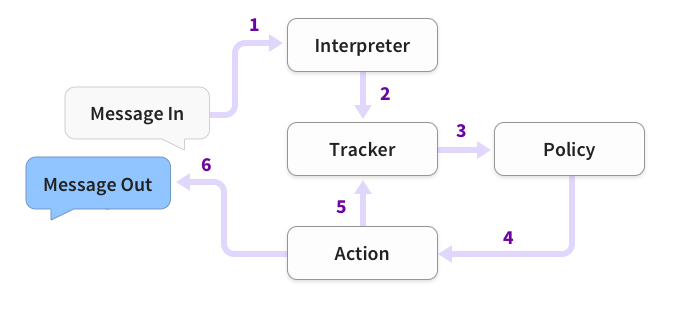
\includegraphics[scale=0.8]{docs/img/project_pics/rasa_message.png}
\centering
\caption{Incoming message processing \cite{dialogflow_overview}}
\label{fig:rasa_msg}
\end{figure}

The steps followed in processing the message are:
\begin{itemize}
    \item The message is received and passed to the Interpreter. It performs several transformations and operations to convert it into a dictionary with the original text, the intent and entities found in it.
    \item The object that keeps track of the conversation state is the Tracker, which receives the info that a new message has arrived
    \item The policy receives the current state of the tracker, and in consequence chooses decides which action to take next.
    \item The chosen action is logged by the tracker, and then sent to the user
\end{itemize}

\section{Conclusions}
In this chapter we have introduced some of the main technologies used in this project and some of the options that we may use.

First of all, we have described the cognitive systems, which is one of the basis of chatbots. We have shown some of the main uses for these systems, as well as some of the most important properties that conform cognitive systems.

After that, we talked about chatbots, gathering information about their origins and the first applications of the technology. After that, we described a brief classification about the different parts that conforms a chatbot, and the task that they perform. Also, we described some of the main frameworks to build chatterbots, presented their main properties and how they work.
\chapter{Architecture and Methodology}
\label{chap:architecture}
\textit{This chapter presents the methodology used in this work. It describes the overall architecture of the project, with the connections between the different components involved on the development of the project.}

\clearpage

\section{Methodology}

\clearpage

\section{Architecture}



\chapter{Case study}
\label{chap:case-study}

\textit{In this chapter we are going to describe a selected use case. This section will discuss the two use case: Sentiment and Emotion Analysis applying Deep Learning techniques, which will include the datasets used, the first steps with the neural networks and the use of more advance techniques.}

\clearpage

\section{Techniques}

\section{Datasets}

\section{Results}
...

\chapter{Conclusions}
\label{chap:conclusions}
\textit{This chapter will describe the achieved goals done by the master thesis following some the key points developed in the project.}

\clearpage
\section{Achieved Goals}

The achieved goals for this project are the following ones:

\begin{itemize}
    \item ...
\end{itemize}

\clearpage
\section{Conclusion}
\label{sec:conclusion}

The project has fulfilled the proposed objectives, but we must refer to each one of these objectives in to draw a general conclusion.




% apendices del proyecto
\appendix
\chapter{Example}

This is the description of the appendix.
\phantomsection
\nocite{*}
\addcontentsline{toc}{chapter}{Bibliography}
%ieeetr
\bibliographystyle{plain}
{
\small
\bibliography{biblio/ref}
}

%\cleardoublepage
\end{document}